\documentclass[journal,11pt]{vgtc}  

\usepackage{mathptmx}
\usepackage{graphicx}
\usepackage{times}
\usepackage{amsmath}
\DeclareMathOperator*{\argmax}{arg\,max}

\usepackage[bookmarks,backref=true,linkcolor=black]{hyperref} %,colorlinks
\hypersetup{
  pdfauthor = {},
  pdftitle = {},
  pdfsubject = {},
  pdfkeywords = {},
  colorlinks=true,
  linkcolor= black,
  citecolor= black,
  pageanchor=true,
  urlcolor = black,
  plainpages = false,
  linktocpage
}

\onlineid{0}


\title{Twitter Trending Topic Classification}
\author{MES: Maria Ludovica Costagliola - Emanuele De Santis - Serena Ferracci}

%% Abstract section.
\abstract{
  \normalsize
  The Web Information Retrieval course allowed us to develope the described project.
  It is about classification of topics that are trending of twitter in a given moment. We have dealt 
  with (i) text based classification using single tweets (ii) network based classification exploiting the 
  graph structure of Twitter. 

  The used dataset is composed by tweets divided by trending topics. 
  We classify the trending topics into 8 categories: \textit{Event, Health, Movie, Music, Politics, Science, Society} and \textit{Sport}.

  The first approach gives good results in terms of precision and recall. Instead, the second approach 
  does not give conclusive results because it requires too many resources to be implemented on a single machine.

} 


\begin{document}


\maketitle

\section{Introduction}
We chose this project because Twitter is one of the most popular social network. 
It is used every day by millions of users expressing their opinions about several fields.
When an user looks for something, the first thing Twitter displays to him is the list of 
trending topics of the moment. Often the user can not know what the topic is about, so it has to manually 
search for tweets belonging to that trending topic to better understand it.

It is interesting for the user to have a way to know what the Trending Topic is about
without further searches.
Our work tries to replicate the results obtained by \cite{lee_palsetia_narayanan_patwary_agrawal_choudhary_2011}.  
The general categories used in this project are 8, named: \textit{Event, Health, Movie, Music, Politics, Science, Society} and \textit{Sport}.


\section{Related Work}
The paper we refer to is the work done by Lee et al. for tweets classification \cite{lee_palsetia_narayanan_patwary_agrawal_choudhary_2011}. 
They have used 18 general categories to classify each trending topic.
They address the problem following two different approaches. The first one is a supervised learning technique, named
Multinomial Naive Bayes. Instead, the second one is network based and it uses Personalized PageRank to compute the 
top-k influencers and then it computes the intersection between the influencers to classify the new trending topic.

All trending topics they used were downloaded from \textit{what the trend}.

\section{Dataset}
Since it was not possible to get a suitable dataset for our purpose, we needed to build it manually
using Twitter APIs \cite{twitter} through Tweepy \cite{api}.

In \texttt{tweets\_retrieve.py} we
first retrieved trending topics from USA using USA WOEID (Where On Earth IDentifier, that is 23424977 for USA). 
Then, for each trending topic, we queried Twitter to get all tweets belonging to the given topic.
We pay attention to retrieve the entire text of the tweet; in case of retweeted statuses we consider only the 
retweeted text. 
Twitter imposes some limitation on GET requests, in particular we could retrieve 180 tweets every 15 minutes.
So, we have to handle exceptions fired due to the reached limit.
In order to submit a request we have to set up Tweepy authorization handler with our
consumer key and our access token we take from our twitter developer account.
As result, we get a file for each tweet where its name is the ID of the author and the body is the text of his tweet.
This file is placed in a folder whose name is composed by the name of the trending topic.
At the end, we collect about 20.000 tweets belonging to 139 trending topics.

After this first phase, we had to retrieve the link structure for the users that wrote the tweets collected 
in the previous phase. In order to do so, we developed two python files, named \texttt{followers\_retrieve.py} and 
\texttt{friends\_retrieve.py}. 
We used Tweepy to retrieve all followers and friends for each author ID being aware of all exceptions.
Since the limitation, in this case, is 15 queries every 15 minutes, we had to find a way to speed up the process.
To do so we decided to parallelize the computation using more than one key (precisely 6 keys), contrarily with respect to the previous 
retrieving phase, and working in data separation. We associated each key to a subset of IDs to be processed, this
mapping was done using a simple hash function. 
We saved the list of followers and the list of friends for an user $x$ in the files named \texttt{x - followers.txt}
and \texttt{x - friends.txt}. These two files are saved in the same folder that contains the tweet tweeted by $x$.

We faced three main problems to retrieve the dataset:
\begin{itemize}
  \item some users changed their privacy settings between the first and the second phase
  of our retrieving. For this reason we couldn't get neither their followers nor their friends.
  \item a subset of users have a plethora of followers, of the order of millions of users. 
  It took a lot of time to complete the retrieving of their followers, sometimes almost an 
  entire day at full capacity.
  It also happened that the execution stopped due to connection problems or other unpredictable events, 
  so it was not possible to retrieve the entire list of IDs.
  \item there wasn't a retrievable ground-truth for the trending topics we collected.
\end{itemize}

The last problem was the only one that we could manage to solve. 

We tried to automatically get a classification using some pretrained machine learning algorithms, but when we 
manually checked the classification done, we saw that almost all the predictions were wrong.

The solution that we came up with was to label every trending topic by hand. 
We took one directory at a time, we read some tweets to understand what the topic was about, 
we assigned to the directory a single category among the 8 defined.

\section{Classification using Naive Bayes}
Multinomial Naive Bayes is a very useful Machine Learning algorithm when we are dealing with
text classification. 
Naive Bayes is based on the assumption that the probability that a document (composed of terms $(t_1,...,t_T)$) belongs to a class $c_k$
, namely $P(c_k | t_1, ..., t_T) $, can be written as $P(c_k) \cdot \prod\limits_{i=1}^{T}P(t_i)$.
The probability that a term is in a class is conditionally independent from the probability that 
 another term is in the same class.

 So Naive Bayes classifier makes a prediction $\hat{y}$ using the following formula

\begin{center}
$\hat{y} = \argmax\limits_{k \in \{1, ..., K \}} P(c_k) \cdot \prod\limits_{i = 1}^{T} P(t_i | c_k)$
\end{center}

We rearranged the data in the dataset in order to have a folder that contains 8 subfolders (one for each
category we considered). Each one contains all the tweets belonging to a trending topic that belongs to the category of the subfolder.
This operation is done by \texttt{training\_set.py} python script.

We developed also \texttt{naive\_bayes\_no\_stemmming.py}. It takes as dataset the folder yet mentioned.

\texttt{sklearn} allows to make an automatic division of the dataset, splitting it into train set and
test set (25\% for the test set).
The training set was converted first computing the corresponding tf-idf matrix through the \texttt{TfidfVectorizer} function. 
This is then used to actually transform the original dataset into the term-document matrix.
The term-document matrix is used by the Multinomial Naive Bayes classifier to execute the learning process.

After the learning phase, we needed to evaluate the performances of the classifier: we applied the same transformation as before
to the test set and we made the algorithm predict these instances. We get at the end the following results:

\begin{figure}[h]
 \centering
 \includegraphics[scale=0.5]{naive_bayes_no_stemming}
 \caption{Classification evaluation without applying stemming}
 \label{no-stemming}
\end{figure}

We tried, also, another version of the program, \texttt{naive\_bayes\_stemming.py}, where we used the stemming technique:
we tokenized each word, applying an \texttt{EnglishStemmer} from \texttt{nltk} \cite{nltk}.
Making the vectorization phase together with stemming, we get the results shown in \ref{stemming}.

\begin{figure}[h]
 \centering
 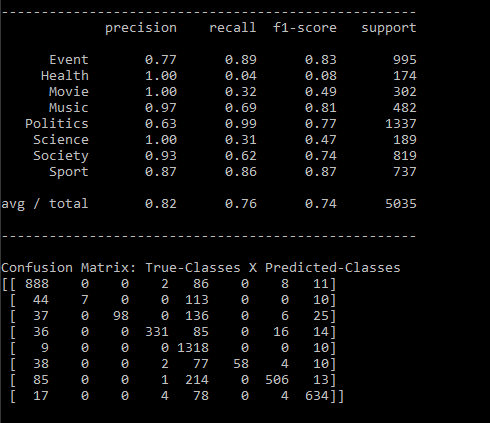
\includegraphics[scale=0.5]{naive_bayes_stemming}
 \caption{Classification evaluation applying stemming to the training set}
 \label{stemming}
\end{figure}

As we can see from \ref{no-stemming} and \ref{stemming}, we get lower results using stemming technique. Usually, stemming reduces the size of the particular vocabulary in order to increase performances of the classifier. In our case, this didn't happen since our tweets are written not only in English, but also in Spanish. So, it's not possible to apply this preprocessing technique since it bases its computation according to the language of the target vocabulary, that must be unique.

\newpage
\section{Network Based Classification}
For this second approach, we exploited the structure of the social network. We assumed that if there is a significant overlap among users 
generating tweets on two topics, then it implies a close relationship between these two topics.
Network-based data modeling uses the categories that are manually labeled in the previous approach to predict
the category of a new trending topic.

To compute the network based classification, we first had to construct the directed graph, that represents a small 
subset of the Twitter's network. 
In the directed graph every node represents an user and every edge represents a relationship between two users.
If a node has an incoming edge, meaning it is followed by another node, we call the last one follower. Instead, if a node has an 
outgoing edge, meaning that it follows another node, we call the last one friend.
To construct the described graph, we developed the python file \texttt{pagerank\_learning.py}, in which we used the predefined library \texttt{NetworkX}. The library offers to the programmer 
several functions that facilitate the construction of the graph. 
Once the graph is finalized, we compute the PageRank using a function present in the mentioned library. 
This function takes as parameter only the graph defined as describe above and returns a dictionary of nodes 
with the PageRank as value.
 
The purpose of this computation is to find the top-k influencers for each category. The top influencers
are the ones that have the higher PageRank value.
For every category, the program runs independently from previous executions. Each time we save in a 
distinct file the top-k influencers of that category. The name of the file is 
\texttt{topk.txt} and it is placed in the subfolder of that particular category in the training set folder.
After the retrieve of the influencers for each category, the training is complete. 

In order to perform the classification of a new trending topic, we proceeded as follows. 
We had to construct a distinct directed graph also for the new topic. The procedure is the same as the one performed
to build the other directed graphs. Once the graph was complete, we executed the PageRank on it. 
As result we had the top-k influencers of this particular trending topic. 

At this point, we took the influencers computed in the training phase and the influencers computed in the
last phase and we started to compute the intersection between the top-k influencers of the new topic and 
all other sets of influencers. 
The result of the intersection will be the number of users that wrote a tweet about the new topic and, also, 
a tweet about the analyzed category. 
Once we had completed all the intersection, we order in descending order the categories according to the 
value obtained with the intersection. The category with the highest value it is the category
to which the new topic is assigned.
By performing what it has just been described, we have obtained the following results:


\bibliographystyle{abbrv}
%%use following if all content of bibtex file should be shown
%\nocite{*}
\bibliography{template}
\end{document}
